\documentclass[10pt]{article}
\usepackage[margin=0.8in]{geometry}
\usepackage{amsmath}
\usepackage{graphicx}
\usepackage{tikz}
\usetikzlibrary{
	decorations.pathmorphing,
	decorations.markings,
	positioning,
	arrows.meta,
	calc,
	shapes.geometric
}
\usepackage{tabularx}
\usepackage{booktabs}

\title{PID Control: Concepts, Simulation, and Practical Implementation}
\author{Gaurav Upreti}
\date{November 12, 2026}

\begin{document}
	
	\maketitle
	
	\section{Introduction}
	A \textbf{controller} is the ``brain'' of an automated system. It regulates a piece of hardware by repeating the same three steps again and again:
	\begin{enumerate}
		\item \textbf{Measure:} use a sensor to read the variable we care about (a speed, a position, an angle, a temperature).
		\item \textbf{Compare:} calculate the \textbf{error}, the difference between where we want to be (the target) and where we are right now:
		\begin{equation}
			\text{error} = \text{target} - \text{actual value}.
		\end{equation}
		\item \textbf{Act:} adjust the machinery in proportion to that error, so that the gap shrinks.
	\end{enumerate}
	Because this cycle repeats many times per second, the gap is reduced a little at every step until the actual value reaches the target.
	
	\subsection{A daily-life example: running to a spot in a field}
	Imagine you are running across a field to reach a marked spot and stop exactly on it. You are acting as a controller:
	\begin{itemize}
		\item \textbf{Sensor:} your eyes, which tell you how far away the spot is.
		\item \textbf{Error:} the remaining distance to the spot.
		\item \textbf{Actuator:} your legs, which set your running speed.
	\end{itemize}
	Every few strides you look up and check how far you still are. When the spot is far away (large error), you run fast. As you get closer (smaller error), you slow down. When the error is almost zero, you are nearly walking, and you stop right on the spot. If you ran at full speed the whole way, you would overshoot, which is exactly what happens to a machine when its controller reacts too strongly.
	
	\subsection{The feedback loop}
	Figure~\ref{fig:general_control} shows the cycle as a loop. Information flows from the target, through the controller and the machine, and returns through the sensor to be compared with the target again. This return path is called \textbf{feedback}.
	
	\begin{figure}[ht]
		\centering
		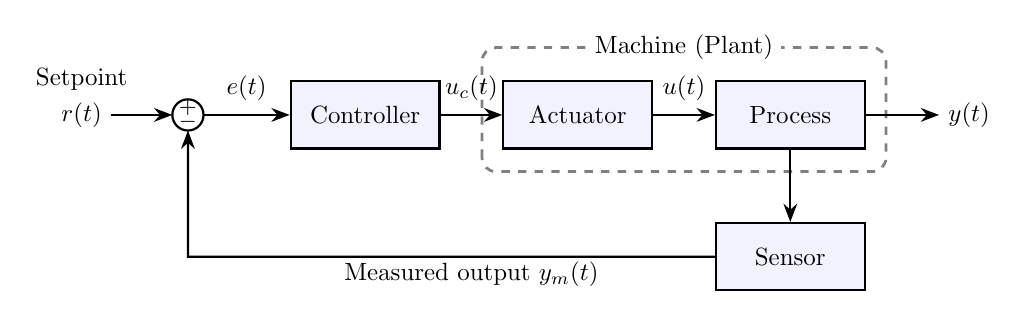
\begin{tikzpicture}[
			>=Stealth,
			thick,
			scale=0.9,
			transform shape,
			block/.style={
				draw,
				rectangle,
				minimum width=2.1cm,
				minimum height=0.95cm,
				align=center,
				fill=blue!5
			}
			]
			% Setpoint
			\node at (0,0) (ref) {$r(t)$};
			\node at (0,0.5) {Setpoint};
			
			% Summing junction
			\draw (1.5,0) circle (0.22);
			\node at (1.5,0.1) {\small $+$};
			\node at (1.5,-0.1) {\small $-$};
			
			% Controller
			\node[block] (controller) at (4,0) {Controller};
			
			% Plant enclosure
			\draw[dashed, rounded corners=5pt, gray, line width=1pt]
			(5.65,-0.8) rectangle (11.35,0.95);
			\node[fill=white,inner sep=3pt] at (8.5,0.95) {Machine (Plant)};
			
			% Actuator
			\node[block] (actuator) at (7,0) {Actuator};
			
			% Process
			\node[block] (process) at (10,0) {Process};
			
			% Forward path
			\draw[->] (ref) -- (1.28,0);
			\draw[->] (1.72,0) -- node[above=2pt] {$e(t)$} (controller.west);
			\draw[->] (controller.east) -- node[above=2pt] {$u_c(t)$} (actuator.west);
			\draw[->] (actuator.east) -- node[above=2pt] {$u(t)$} (process.west);
			\draw[->] (process.east) -- (12.1,0) node[right] {$y(t)$};
			
			% Sensor
			\node[block] (sensor) at (10,-2.0) {Sensor};
			\draw[->] (process.south) -- (sensor.north);
			
			% Feedback path
			\draw[->] (sensor.west) -- (1.5,-2.0) -- (1.5,-0.22);
			\node at (5.5,-2.25) {Measured output $y_m(t)$};
		\end{tikzpicture}
		\caption{The feedback loop: the target is compared with the sensor reading, the error drives the controller, and the controller drives the machine.}
		\label{fig:general_control}
	\end{figure}
	
	\section{PID Formulation}
	At every moment a PID controller measures the \textbf{error}, the gap between the target (setpoint) $r(t)$ and the measured value $y(t)$:
	\begin{equation}
		e(t) = r(t) - y(t).
	\end{equation}
	The controller computes an output $u(t)$ which is the sum of three terms:
	\begin{equation} 
		u(t) = \underbrace{K_p\,e(t)}_{\text{P: present}} + \underbrace{K_i \int_{0}^{t} e(\tau)\,d\tau}_{\text{I: past}} + \underbrace{K_d\, \frac{de(t)}{dt}}_{\text{D: future trend}} .
		\label{eq:pid} 
	\end{equation}
	
	\begin{table}[h]
		\centering
		\small
		\begin{tabular}{llll}
			\toprule
			Symbol & Meaning & Unit (for position control) & Role \\
			\midrule
			$e(t)$ & error, target minus actual & m & measures current gap \\
			$u(t)$ & controller output (force) & N & drives the actuator \\
			$K_p$ & proportional gain & N/m & reacts to the \emph{present} error \\
			$K_i$ & integral gain & N/(m$\cdot$s) & reacts to the \emph{accumulated past} error \\
			$K_d$ & derivative gain & N$\cdot$s/m & reacts to \emph{how fast} the error changes \\
			$\tau$ & dummy time variable inside the integral & s & integration variable \\
			\bottomrule
		\end{tabular}
		\caption{Variables and units in the PID formulation.}
	\end{table}
	
	\paragraph{P (present):} Push in proportion to how far we are from the target. A large error gives a large push. Larger $K_p$ gives a faster response, but too much causes overshoot and oscillation.
	\paragraph{I (past):} Add up the error over time. If a small error persists, the integral keeps growing and pushes harder until the error is removed. This is what eliminates the final offset left by P alone.
	\paragraph{D (rate of change):} Look at how quickly the error is changing. If the error is shrinking fast, D reduces the push to brake the motion before overshooting. It acts like damping.
	
	\begin{figure}[ht]
		\centering
		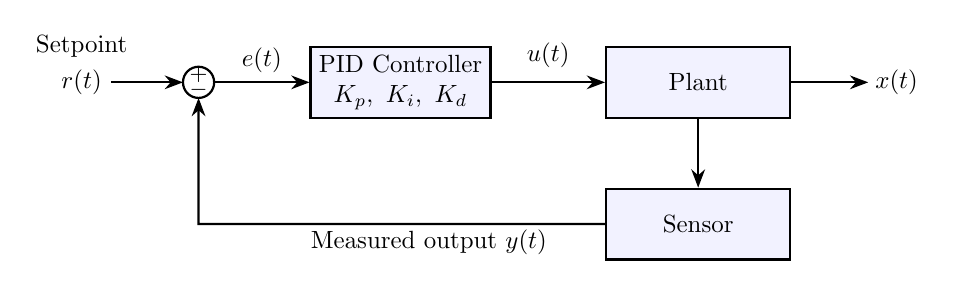
\begin{tikzpicture}[
			>=Stealth,
			thick,
			scale=0.9,
			transform shape,
			block/.style={
				draw,
				rectangle,
				minimum width=2.4cm,
				minimum height=1.0cm,
				align=center,
				fill=blue!5
			}
			]
			\node at (0,0) (ref) {$r(t)$};
			\node at (0,0.5) {Setpoint};
			
			\draw (1.65,0) circle (0.22);
			\node at (1.65,0.1) {\small $+$};
			\node at (1.65,-0.1) {\small $-$};
			
			\node[block] (pid) at (4.5,0) {PID Controller\\$K_p,\ K_i,\ K_d$};
			\node[block,minimum width=2.6cm] (plant) at (8.7,0) {Plant};
			\node at (11.5,0) (out) {$x(t)$};
			
			\draw[->] (ref) -- (1.43,0);
			\draw[->] (1.87,0) -- node[above] {$e(t)$} (pid.west);
			\draw[->] (pid.east) -- node[above=2pt] {$u(t)$} (plant.west);
			\draw[->] (plant.east) -- (11.1,0);
			
			\node[block,minimum width=2.6cm] (sensor) at (8.7,-2.0) {Sensor};
			\draw[->] (plant.south) -- (sensor.north);
			\draw[->] (sensor.west) -- (1.65,-2.0) -- (1.65,-0.22);
			\node at (4.9,-2.25) {Measured output $y(t)$};
		\end{tikzpicture}
		\caption{Closed-loop PID control system.}
		\label{fig:pid_control}
	\end{figure}
	
	\subsection{The version a computer runs}
	A computer works in small time steps of length $\Delta t$ (the sampling period). At step $k$ the integral becomes a running sum and the derivative becomes a finite difference:
	\begin{align}
		e_k &= r_k - y_k, \\
		I_k &= I_{k-1} + e_k\, \Delta t, \\
		D_k &= \frac{e_k - e_{k-1}}{\Delta t}, \\
		u_k &= K_p\, e_k + K_i\, I_k + K_d\, D_k .
		\label{eq:pid-discrete}
	\end{align}
	Each cycle the program (1) reads the sensor, (2) computes $e_k$, (3) updates $I_k$ and $D_k$, (4) sends $u_k$ to the actuator, and (5) waits for the next step.
	
	\section{The Test System}
	We control a block of mass $m$ attached to a spring and a damper, similar to a car suspension. The \textbf{block slides horizontally on a frictionless surface}, so gravity acts perpendicular to the motion and does not affect the dynamics. The spring is at its natural length at $x=0$, and a positive force $u$ pushes the block toward positive $x$. The goal is to move the block to $x = r = 1$\,m.
	
	\begin{table}[h]
		\centering
		\small
		\begin{tabular}{lll}
			\toprule
			Parameter & Value & Unit \\
			\midrule
			Mass $m$ & 1 & kg \\
			Damping $c$ & 10 & N$\cdot$s/m \\
			Spring stiffness $k$ & 20 & N/m \\
			Target $r$ & 1 & m \\
			\bottomrule
		\end{tabular}
		\caption{Parameters of the test system.}
	\end{table}
	
	\begin{figure}[ht]
		\centering
		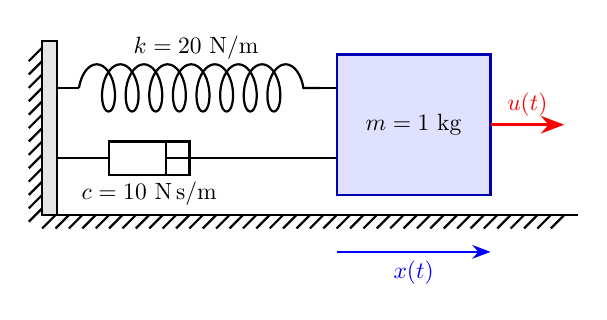
\begin{tikzpicture}[
			>=Stealth,
			thick,
			scale=0.85,
			transform shape,
			spring/.style={
				decorate,
				decoration={coil, aspect=0.5, segment length=3mm, amplitude=3mm}
			}
			]
			\draw[fill=gray!20] (0,0) rectangle (0.22,2.6);
			\foreach \y in {0.1,0.3,...,2.5} \draw (0,\y) -- (-0.2,\y-0.2);
			\draw (0,0) -- (8,0);
			\foreach \x in {0.2,0.4,...,7.8} \draw (\x,0) -- (\x-0.2,-0.2);
			
			\draw (0.22,1.9) -- (0.55,1.9);
			\draw[spring] (0.55,1.9) -- (4.15,1.9);
			\draw (4.15,1.9) -- (4.4,1.9);
			\node[above] at (2.3,2.2) {$k=20\ \mathrm{N/m}$};
			
			\draw (0.22,0.85) -- (1.0,0.85);
			\draw (1.0,0.6) rectangle (2.2,1.1);
			\draw (1.85,0.6) -- (1.85,1.1);
			\draw (1.85,0.85) -- (4.4,0.85);
			\node at (1.6,0.32) {$c=10\ \mathrm{N\,s/m}$};
			
			\draw[fill=blue!12, draw=blue!70!black] (4.4,0.3) rectangle (6.7,2.4);
			\node at (5.55,1.35) {$m=1\ \mathrm{kg}$};
			
			\draw[->,red,very thick] (6.7,1.35) -- (7.8,1.35);
			\node[above,red] at (7.25,1.35) {$u(t)$};
			
			\draw[->,blue,thick] (4.4,-0.55) -- (6.7,-0.55);
			\node[below,blue] at (5.55,-0.55) {$x(t)$};
		\end{tikzpicture}
		\caption{Horizontal mass--spring--damper system.}
		\label{fig:mass_spring_damper}
	\end{figure}
	
	\subsection{Equation of motion}
	Newton's second law (mass times acceleration equals the sum of forces) gives
	\begin{equation}
		m\,\ddot{x}(t) + c\,\dot{x}(t) + k\,x(t) = u(t)
		\quad\Longrightarrow\quad
		\ddot{x} = u - 10\,\dot{x} - 20\,x .
		\label{eq:plant}
	\end{equation}
	Here $x$ is position (m), $\dot{x}$ is velocity (m/s), $\ddot{x}$ is acceleration (m/s$^2$), $c\dot{x}$ is the damper force, and $kx$ is the spring force. For simulation we write this as two first-order equations with state $(x, v)$, where $v=\dot{x}$:
	\begin{equation}
		\dot{x} = v, \qquad
		\dot{v} = \frac{1}{m}\bigl(u - c\,v - k\,x\bigr).
	\end{equation}
	Taking the Laplace transform with zero initial conditions gives the transfer function
	\begin{equation}
		G(s) = \frac{X(s)}{U(s)} = \frac{1}{m s^2 + c s + k} = \frac{1}{s^2 + 10 s + 20}.
	\end{equation}
	
	\subsection{Why the spring needs a constant push}
	Suppose the block is at rest at the target, so $\dot{x}=0$ and $\ddot{x}=0$. The damper force is zero because there is no motion, and Eq.~\eqref{eq:plant} reduces to
	\begin{equation}
		k\,x = u \quad\Longrightarrow\quad u_{\text{hold}} = k\, r = 20 \times 1 = 20\ \text{N}.
	\end{equation}
	The stretched spring pulls the block back with 20\,N, so the actuator must push forward with a constant 20\,N to hold it at 1\,m. Without this constant force the block drifts back to $x=0$. This explains why P-only control suffers a steady-state offset (Section~5) and why the integral term is required.
	
	\subsection{Open-loop behaviour}
	The \emph{DC gain} is $G(0) = 1/k = 0.05$\,m/N. The natural frequency and damping ratio are
	\begin{equation}
		\omega_n = \sqrt{k/m} = \sqrt{20} \approx 4.47\ \text{rad/s}, \qquad
		\zeta = \frac{c}{2\sqrt{km}} = \frac{10}{2\sqrt{20}} \approx 1.12 .
	\end{equation}
	Since $\zeta > 1$ the open-loop plant is overdamped: left alone it moves smoothly to its final value without oscillating (poles at $s = -5 \pm \sqrt{5} \approx -2.76$ and $-7.24$\,s$^{-1}$). Any oscillation or overshoot seen later is caused by the controller, not by the plant.
	
	\section{How to Judge a Result}
	A controller is judged on its \textbf{step response}: the target jumps from 0 to $r = 1$\,m at $t=0$ and we measure four quantities (Figure~\ref{fig:metrics}):
	\begin{enumerate}
		\item \textbf{Rise time $T_r$} (speed): the time taken to rise from 10\% to 90\% of the target (0.1\,m to 0.9\,m). Smaller is faster. If $y$ never reaches 0.9\,m we record ``never''.
		\item \textbf{Overshoot $M_p$} (how far past the target):
		\begin{equation}
			M_p = \max\!\left(0,\ \frac{y_{\max} - r}{r}\right) \times 100\%.
		\end{equation}
		\item \textbf{Settling time $T_s$} (how long until calm): the time after which the output stays permanently inside the $\pm 2\%$ band around the target ($|e| \le 0.02$\,m).
		\item \textbf{Steady-state error $e_{ss}$} (where it finally stops): the remaining error at the end of the run, $e_{ss} = r - y(t_{\text{end}})$.
	\end{enumerate}
	
	\begin{figure}[ht]
		\centering
		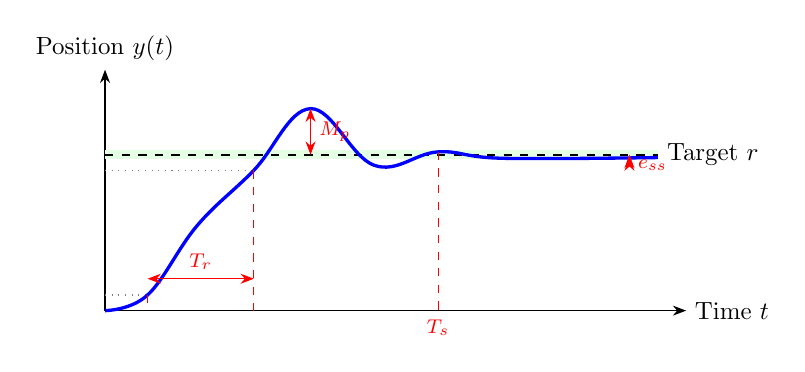
\begin{tikzpicture}[scale=0.9, transform shape, >=Stealth]
			\draw[->] (0,0) -- (8.2,0) node[right] {Time $t$};
			\draw[->] (0,0) -- (0,3.4) node[above] {Position $y(t)$};
			
			% Target and 2% band
			\fill[green!10] (0,2.14) rectangle (7.8,2.26);
			\draw[dashed, thick] (0,2.2) -- (7.8,2.2) node[right] {Target $r$};
			\draw[dotted, gray] (0,1.98) -- (2.1,1.98); % 90%
			\draw[dotted, gray] (0,0.22) -- (0.6,0.22); % 10%
			
			% Step response curve
			\draw[very thick, blue] plot [smooth, tension=0.65] coordinates {
				(0,0) (0.6,0.22) (1.3,1.2) (2.1,1.98) (2.9,2.85) (3.8,2.05) (4.7,2.24) (5.6,2.15) (7.8,2.16)
			};
			
			% Rise time Tr
			\draw[dashed, red] (0.6,0.22) -- (0.6,0);
			\draw[dashed, red] (2.1,1.98) -- (2.1,0);
			\draw[<->, red] (0.6,0.45) -- (2.1,0.45) node[midway, above, font=\footnotesize] {$T_r$};
			
			% Overshoot Mp
			\draw[<->, red] (2.9,2.2) -- (2.9,2.85) node[midway, right, font=\footnotesize] {$M_p$};
			
			% Settling time Ts
			\draw[dashed, red] (4.7,2.24) -- (4.7,0) node[below, font=\footnotesize] {$T_s$};
			
			% Steady-state error ess
			\draw[<->, red] (7.4,2.16) -- (7.4,2.2);
			\node[right, red, font=\footnotesize] at (7.4,2.05) {$e_{ss}$};
		\end{tikzpicture}
		\caption{The four step-response metrics: rise time $T_r$ (10\%--90\%), peak overshoot $M_p$, $\pm 2\%$ settling time $T_s$, and steady-state error $e_{ss}$.}
		\label{fig:metrics}
	\end{figure}
	
	All measures are computed relative to the \emph{target}, not relative to where the output settles. Thus a P-only controller that stops below 1\,m has a large steady-state error even when its overshoot is 0\%.
	
	\section{Each Part Alone}
	All runs below use the test system of Section~3 with a step to $r=1$\,m, a time step of $\Delta t = 0.01$\,s, and a 5\,s simulation duration.
	
	\subsection{P only}
	Setting $u = K_p e$ in Eq.~\eqref{eq:plant} at equilibrium ($\dot{x}=\ddot{x}=0$) yields:
	\begin{equation}
		K_p (r - x_{ss}) = 20\,x_{ss}
		\;\Longrightarrow\;
		x_{ss} = \frac{K_p}{20 + K_p}\, r,
		\qquad
		e_{ss} = \frac{20}{20 + K_p}\, r .
		\label{eq:pss}
	\end{equation}
	\textbf{Why P alone stops short:} holding the block at $1$\,m requires $20$\,N. A proportional controller generates force only when $e \neq 0$, so it must maintain an error of $e_{ss} = 20/K_p$ to supply that $20$\,N force. Increasing $K_p$ shrinks the error but induces oscillations.
	
	\begin{figure}[h]
		\centering
		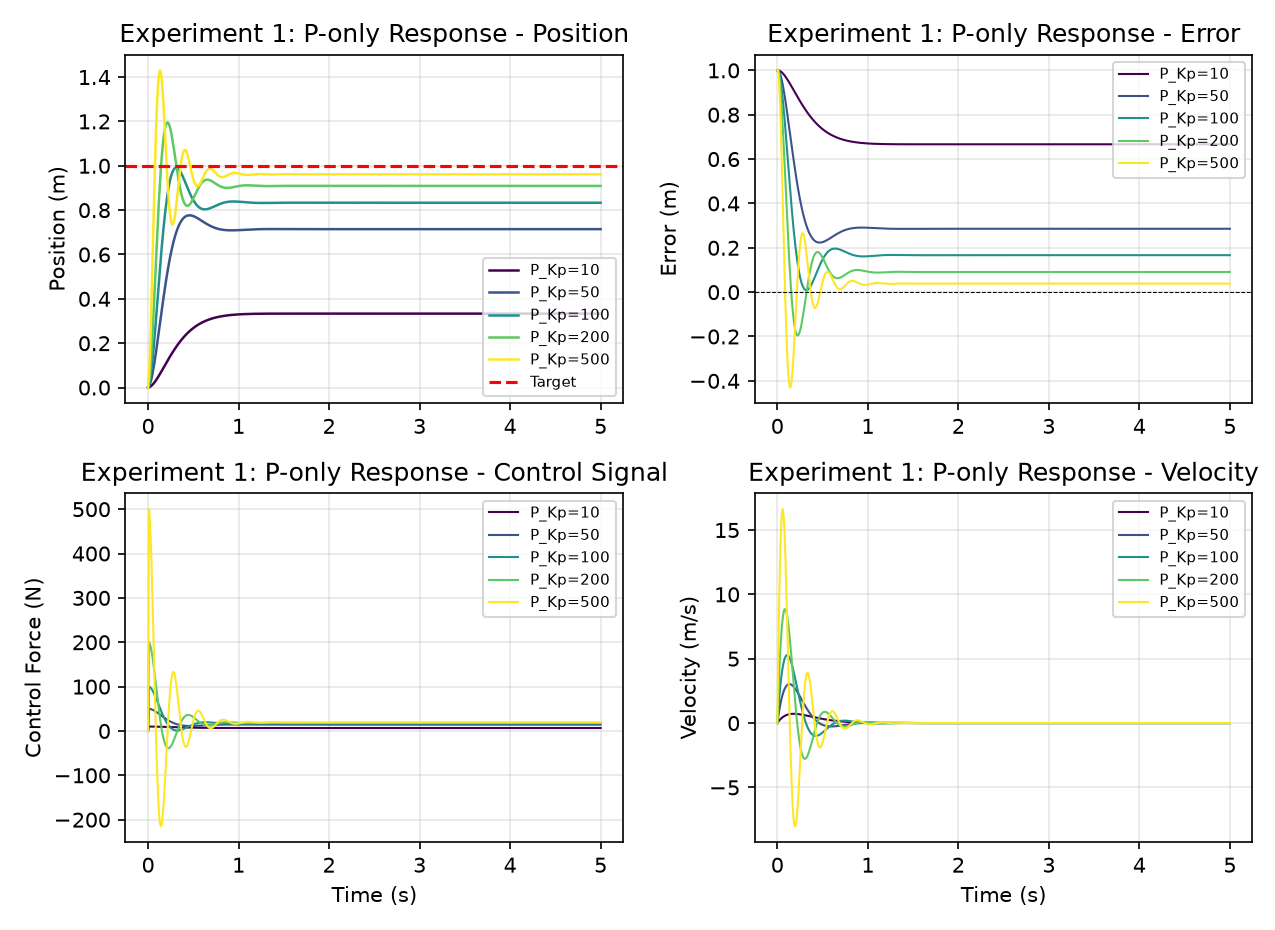
\includegraphics[width=0.78\linewidth]{../experiment_plots/exp1_p_only.png}
		\caption{P-only step responses for $K_p = 10, 50, 100, 200, 500$\,N/m. Every curve settles below the 1\,m target; larger $K_p$ reduces the steady-state offset at the cost of stronger oscillation.}
	\end{figure}
	
	\begin{table}[h]
		\centering
		\small
		\begin{tabular}{@{}rrrrrr@{}}
			\toprule
			$K_p$ (N/m) & Predicted $x_{ss}$ (m) & Predicted $e_{ss}$ (m) & Measured $e_{ss}$ (m) & Rise time $T_r$ (s) & Overshoot $M_p$ (\%) \\
			\midrule
			10  & 0.333 & 0.6667 & 0.6667 & never & 0.0 \\
			50  & 0.714 & 0.2857 & 0.2857 & never & 0.0 \\
			100 & 0.833 & 0.1667 & 0.1667 & 0.18  & 0.0 \\
			200 & 0.909 & 0.0909 & 0.0909 & 0.10  & 19.5 \\
			500 & 0.962 & 0.0385 & 0.0385 & 0.05  & 43.0 \\
			\bottomrule
		\end{tabular}
		\caption{P-only control: analytical prediction from Eq.~\eqref{eq:pss} versus simulation output.}
		\label{tab:ponly}
	\end{table}
	
	Table~\ref{tab:ponly} confirms that the simulated steady-state errors match Eq.~\eqref{eq:pss} to four decimal places.
	
	\subsection{Adding I}
	Adding the integral term gives $u = K_p e + K_i\int e\,dt$. As long as $e \neq 0$, the integral continues accumulating until the integral term alone supplies the 20\,N holding force:
	\begin{equation}
		K_i \int_0^{\infty} e\, d\tau = k\,r = 20\ \text{N}.
	\end{equation}
	With $K_p = 100$ and $K_i = 50$, the error at $t=5$\,s drops from $0.1667$\,m (P only) to $0.0165$\,m and continues decaying toward zero, at the cost of $4.8\%$ overshoot see the green PI curve in Figure~\ref{fig:all}.
	
	\subsection{Adding D}
	With P only, the closed-loop characteristic polynomial is $s^2 + 10s + (20+K_p)$, giving damping ratio $\zeta_P = \frac{10}{2\sqrt{20+K_p}}$. Because the derivative term applies a force opposing velocity, it adds directly to the physical damping:
	\begin{equation}
		\zeta_{PD} = \frac{10 + K_d}{2\sqrt{20 + K_p}} .
	\end{equation}
	For $K_p = 100$, increasing $K_d$ from $0$ to $10$ raises $\zeta$ from $0.456$ to $0.913$, suppressing the transient bounce. Setting $K_d = 2\sqrt{120} - 10 \approx 11.9$ achieves critical damping ($\zeta = 1$). Because $\dot{e}=0$ at rest, D does not alter $e_{ss} = 0.1667$\,m.
	As shown by the orange PD curve in Figure~\ref{fig:all}, adding derivative action damps out the transient bounce seen in P-only control while settling at the exact same $0.1667$\,m steady-state error.
	\section{All Together}
	Figure~\ref{fig:all} compares P, PI, PD, and full PID on the same 1\,m step using baseline gains $K_p = 100$, $K_i = 50$, and $K_d = 10$.
	
	\begin{figure}[h]
		\centering
		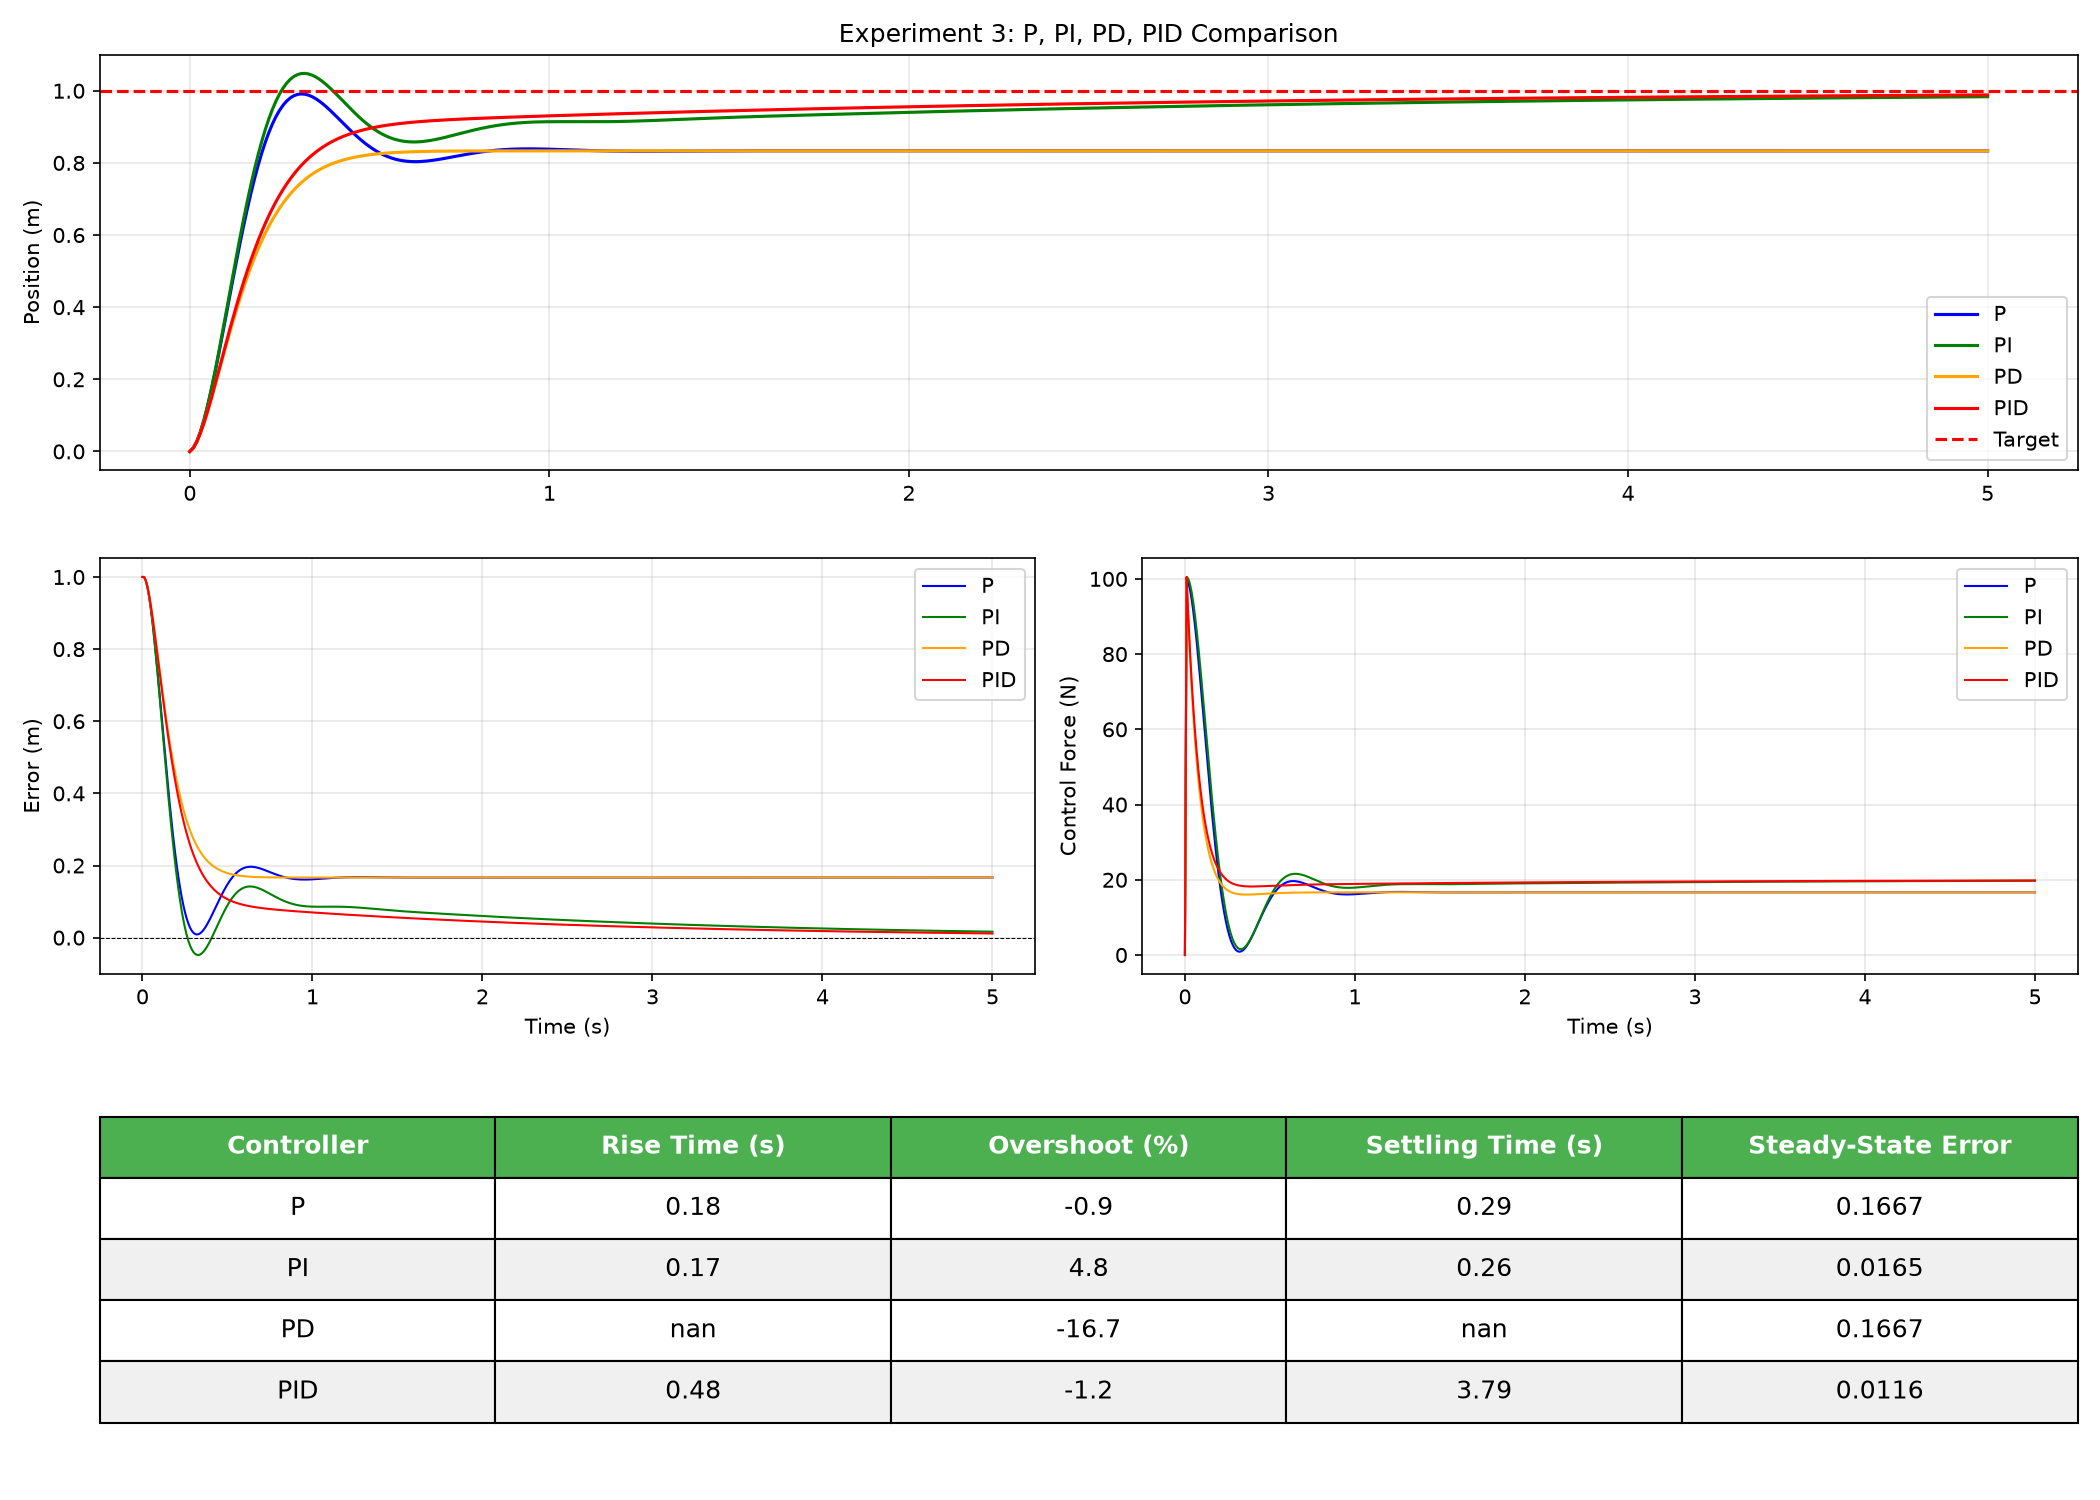
\includegraphics[width=0.82\linewidth]{../experiment_plots/exp3_comparison.png}
		\caption{Step responses and performance metrics of P, PI, PD, and PID with $K_p=100$, $K_i=50$, $K_d=10$.}
		\label{fig:all}
	\end{figure}
	
	Using these baseline gains, full PID eliminates the $16.7\%$ offset of P/PD (reducing $e_{ss}$ to $0.0116$\,m at $t=5$\,s) while keeping overshoot at $0.0\%$ (compared to $4.8\%$ for PI), though its rise time increases to $0.48$\,s due to derivative braking. Systematic gain tuning to speed up this response is covered in Section~8.
	
	
	\paragraph{Chosen reference gains.}
	We select $K_p = 100$, $K_i = 50$, and $K_d = 10$ as our baseline controller because it is the only configuration that simultaneously eliminates steady-state offset ($e_{ss} \to 0$) and achieves $0.0\%$ overshoot, avoiding the $16.7\%$ offset of P/PD and the $4.8\%$ overshoot of PI. Further tuning to speed up its $3.79$\,s settling time is explored in Section~8.
	
	\section{Real-world Problems}
	Real actuators saturate, sensors are noisy, setpoints jump abruptly, and microcontrollers run at finite sampling rates. Below we demonstrate each failure mode on our test system and implement its fix.
	
	\subsection{(a) Integral windup}
	\paragraph{The problem.}
	Our motor can exert at most $\pm 30$\,N. With aggressive gains ($K_p = 100, K_i = 120, K_d = 10$), the controller initially requests well over $30$\,N, saturating the actuator. While the output is clamped at $30$\,N, the error remains positive and the integral term keeps accumulating excess value. When the block reaches $1$\,m, the stored integral forces the block past the target ($10.2\%$ overshoot) until negative error unwinds the accumulator.
	
	\paragraph{The fix: conditional integration (anti-windup).}
	We separate the physical actuator clamp (modeled in the plant) from the controller's internal anti-windup logic: if the candidate theoretical force $u_{\text{raw},k}$ exceeds the known actuator limits $[u_{\min}, u_{\max}]$ \emph{and} the error would push it further into saturation, we freeze the integrator:
	\begin{equation}
		I_k =
		\begin{cases}
			I_{k-1} & \text{if } (u_{\text{raw},k} > u_{\max} \text{ and } e_k > 0) \text{ or } (u_{\text{raw},k} < u_{\min} \text{ and } e_k < 0),\\[2pt]
			I_{k-1} + e_k\,\Delta t & \text{otherwise.}
		\end{cases}
	\end{equation}
	As shown in Figure~\ref{fig:windup}, conditional integration eliminates the windup overshoot completely, reducing $M_p$ from $10.2\%$ down to $0.0\%$.
	
	\begin{figure}[h]
		\centering
		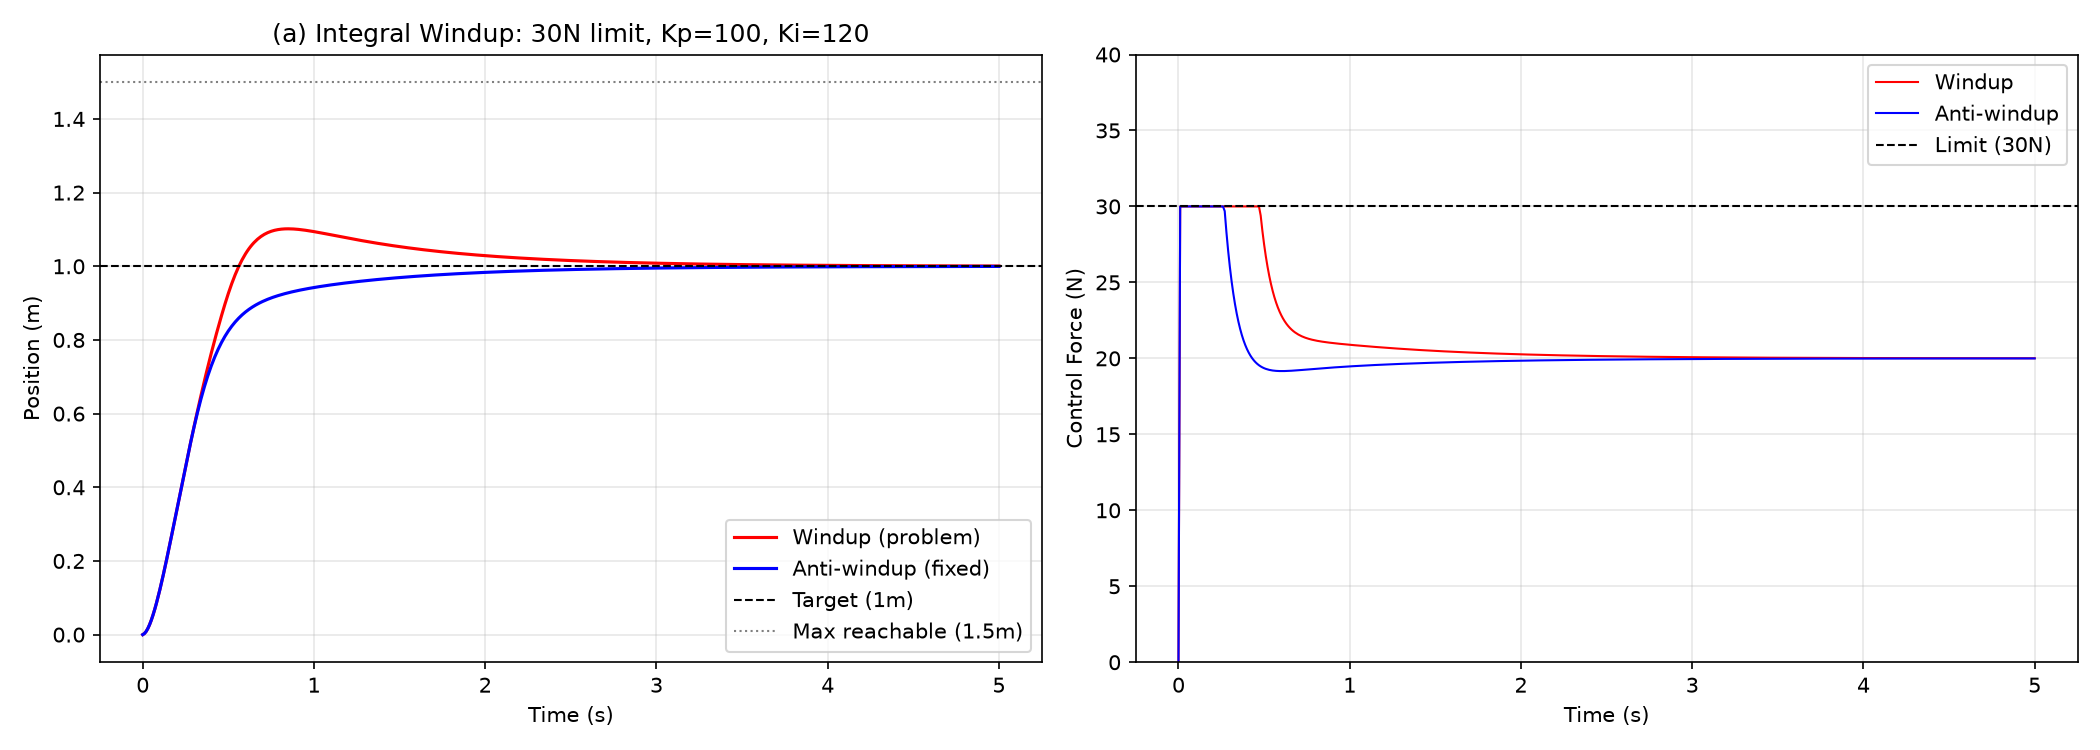
\includegraphics[width=0.82\linewidth]{../experiment_plots/exp4a_windup.png}
		\caption{Integral windup vs.\ conditional integration anti-windup ($\pm 30$\,N actuator limit, $K_p=100, K_i=120, K_d=10$). Overshoot drops from $10.2\%$ to $0.0\%$.}
		\label{fig:windup}
	\end{figure}
	
	\subsection{(b) Sensor noise and the derivative term}
	\paragraph{The problem.}
	Adding Gaussian sensor noise of $\sigma = 1$\,mm ($\pm 1$\,mm) causes severe high-frequency chatter when differentiated over $\Delta t = 0.01$\,s, because $\sigma_{\dot{e}} = \sqrt{2}\sigma / \Delta t \approx 0.141$\,m/s. With $K_d = 50$, the unfiltered control force fluctuates wildly with a standard deviation of $10.12$\,N across the run.
	
	\paragraph{The fix: first-order low-pass filter on D.}
	Filtering the derivative with $\alpha = 0.1$ ($\tau = \Delta t(1-\alpha)/\alpha = 0.09$\,s, cutoff $\approx 1.8$\,Hz):
	\begin{equation}
		D_k^{\text{filt}} = \alpha\, D_k + (1-\alpha)\, D_{k-1}^{\text{filt}}
	\end{equation}
	smooths out the high-frequency noise, reducing the overall control force standard deviation from $10.12$\,N to $7.56$\,N and eliminating steady-state actuator chatter (Figure~\ref{fig:noise}).
	
	\begin{figure}[h]
		\centering
		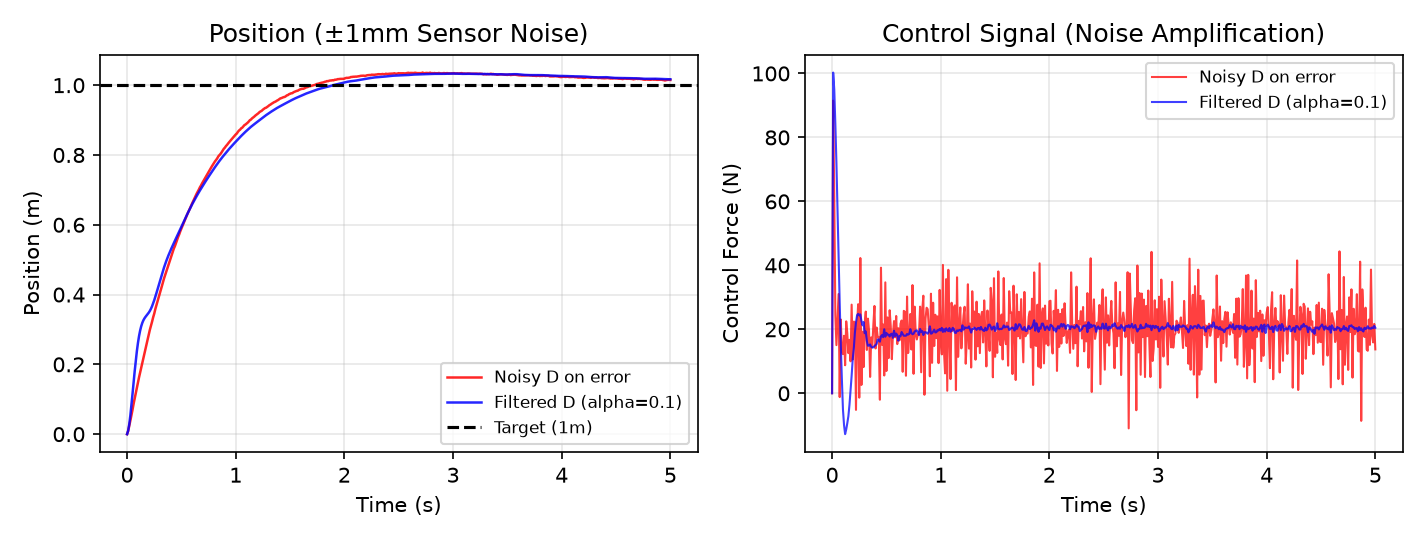
\includegraphics[width=0.82\linewidth]{../experiment_plots/exp4b_noise.png}
		\caption{Effect of $\pm 1$\,mm sensor noise with $K_d=50$. Filtering the derivative ($\alpha=0.1$) suppresses steady-state control chatter, reducing overall control standard deviation from $10.12$\,N to $7.56$\,N.}
		\label{fig:noise}
	\end{figure}
	
	\subsection{(c) Derivative kick}
	\paragraph{The problem.}
	When the target steps suddenly from $1$\,m to $2$\,m at $t=3$\,s, differentiating $e = r - y$ produces a single-step spike of $K_d \Delta r / \Delta t = 10 \times 1 / 0.01 = 1000$\,N. Combined with the P jump ($100$\,N) and holding force ($20$\,N), total requested force spikes to $1120.1$\,N.
	
	\paragraph{The fix: derivative on measurement (PV).}
	Since $\dot{r} = 0$ everywhere except at the instant of a setpoint step, we differentiate the measured position $y$ instead of the error:
	\begin{equation}
		D_k = -K_d\,\frac{y_k - y_{k-1}}{\Delta t}.
	\end{equation}
	As shown in Figure~\ref{fig:kick}, taking D on the process variable drops the peak force from $1120.1$\,N down to $120.1$\,N (leaving only the proportional step $K_p \Delta r = 100$\,N plus the $20$\,N spring force).
	
	\begin{figure}[h]
		\centering
		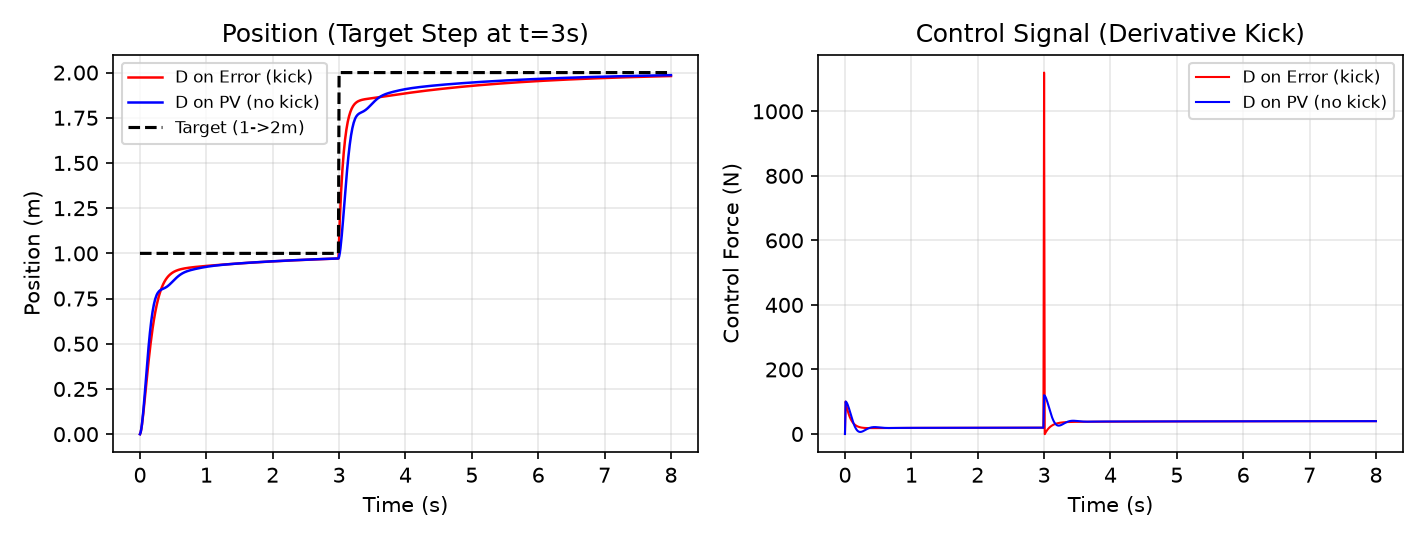
\includegraphics[width=0.82\linewidth]{../experiment_plots/exp4c_kick.png}
		\caption{Target step $1 \to 2$\,m at $t=3$\,s ($K_p=100, K_i=50, K_d=10$). Differentiating on PV cuts the peak control spike from $1120.1$\,N to $120.1$\,N.}
		\label{fig:kick}
	\end{figure}
	
	\begin{figure}[h]
		\centering
		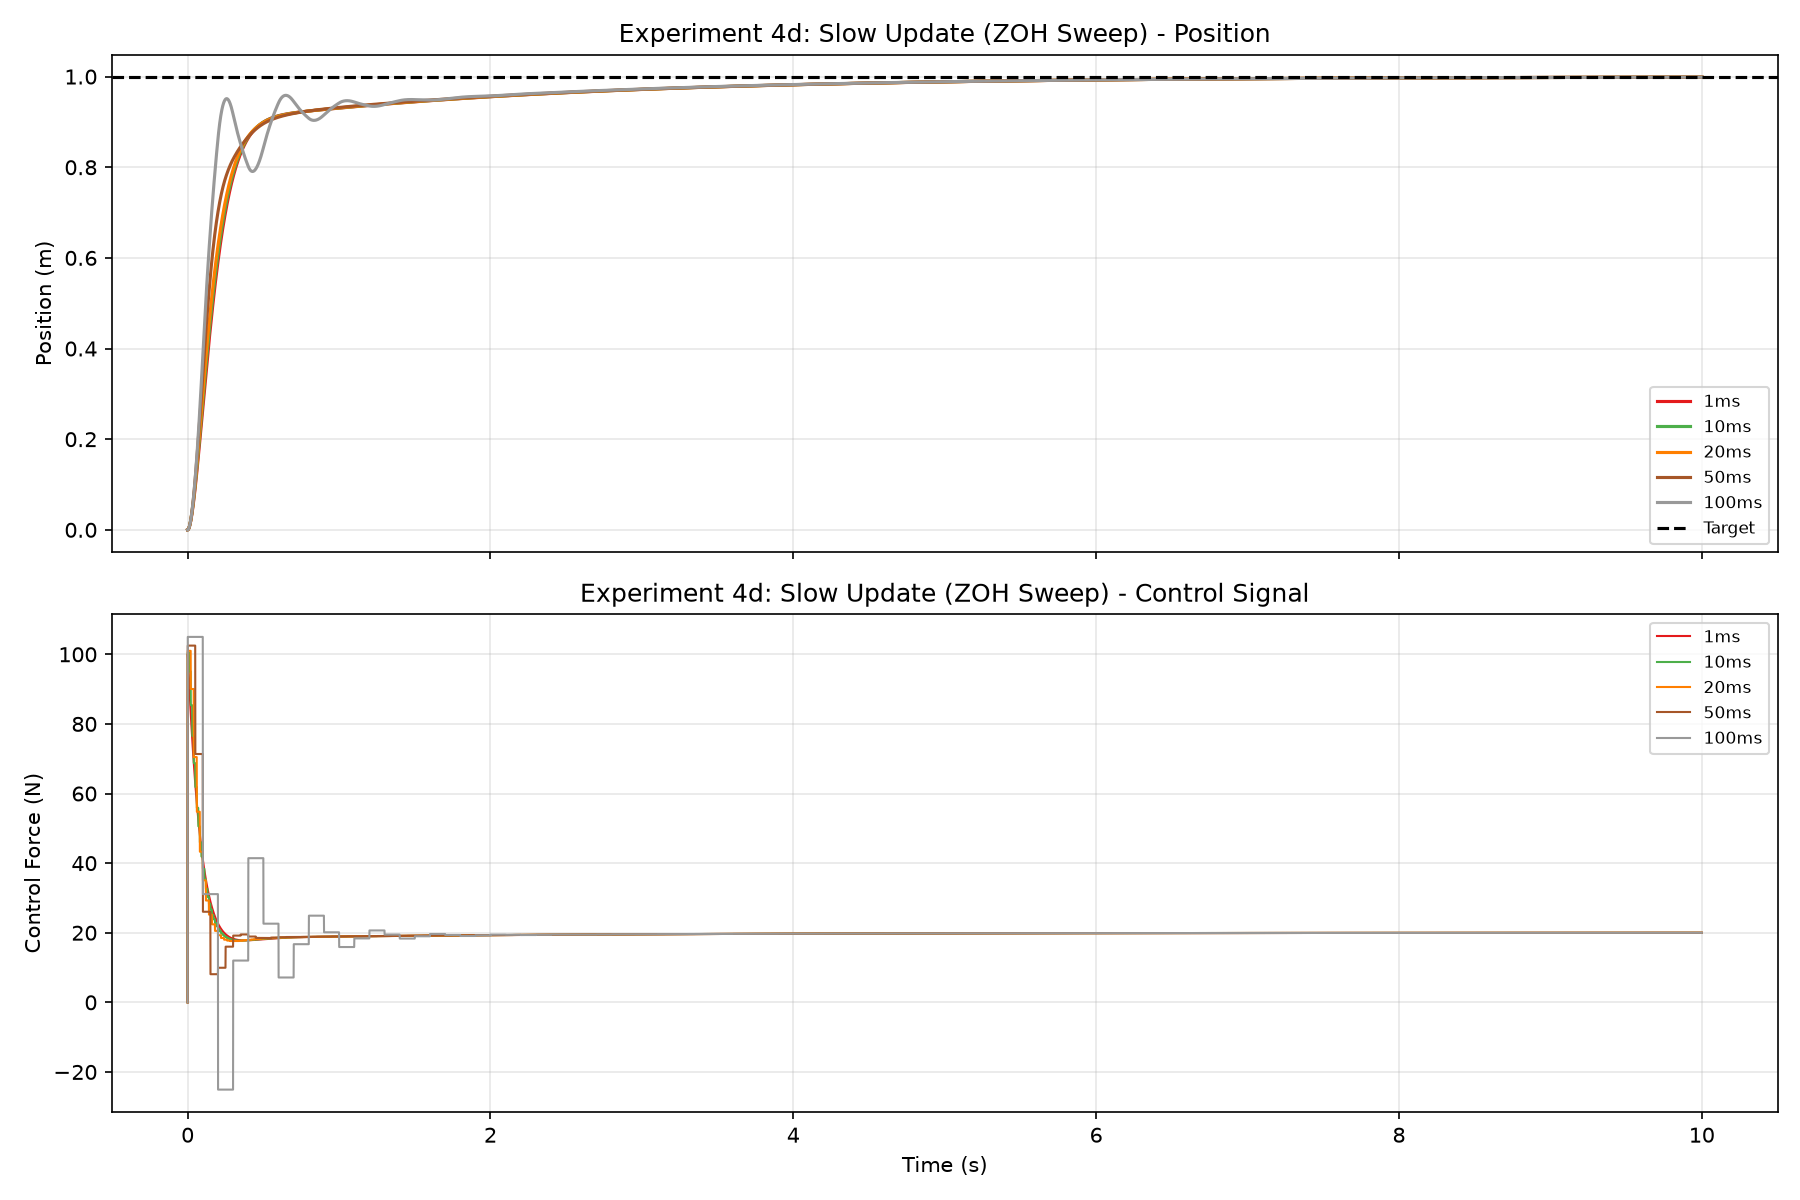
\includegraphics[width=0.82\linewidth]{../experiment_plots/exp4d_zoh.png}
		\caption{Effect of controller sampling period $T_s = 1, 10, 100, 200, 300$\,ms. Up to $100$\,ms the response remains well-damped, whereas at $300$\,ms zero-order hold phase lag drives the system unstable.}
		\label{fig:zoh}
	\end{figure}
	
	\subsection{(d) Slow computer update}
	\paragraph{The problem.}
	Holding the control output constant between updates (zero-order hold, ZOH) over a sampling period $T_s$ introduces an effective phase delay of $T_s/2$, eroding damping. Simulating the plant at $1$\,ms while varying the controller update period $T_s$ yields Table~\ref{tab:ts}.
	
	\begin{table}[h]
		\centering
		\small
		\begin{tabular}{@{}rrr@{}}
			\toprule
			Update time $T_s$ & Overshoot (\%) & Result \\
			\midrule
			1\,ms   & 0.0 & settles in 3.78\,s \\
			10\,ms  & 0.0 & settles in 3.77\,s \\
			50\,ms  & 0.0 & settles in 3.74\,s \\
			100\,ms & 0.0 & settles in 3.70\,s \\
			150\,ms & 11.4 & oscillates, settles in 4.01\,s \\
			200\,ms & 41.6 & still oscillating at 5\,s \\
			250\,ms & 117.5 & large oscillation, growing slowly \\
			300\,ms & --- & unstable (output diverges) \\
			\bottomrule
		\end{tabular}
		\caption{Effect of controller update period $T_s$ ($K_p=100$, $K_i=50$, $K_d=10$).}
		\label{tab:ts}
	\end{table}
	
	\paragraph{The fix.}
	Sample at least 10 times faster than the closed-loop bandwidth. Here, keeping $T_s \le 10$\,ms ($100$\,Hz) preserves continuous-time performance with a wide stability margin.
	

	\section{Choosing the Gains}
	Choosing $K_p$, $K_i$, and $K_d$ is called \emph{tuning}. We can tune either on a mathematical simulation model or directly on physical hardware.
	
	\begin{figure}[t]
		\centering
		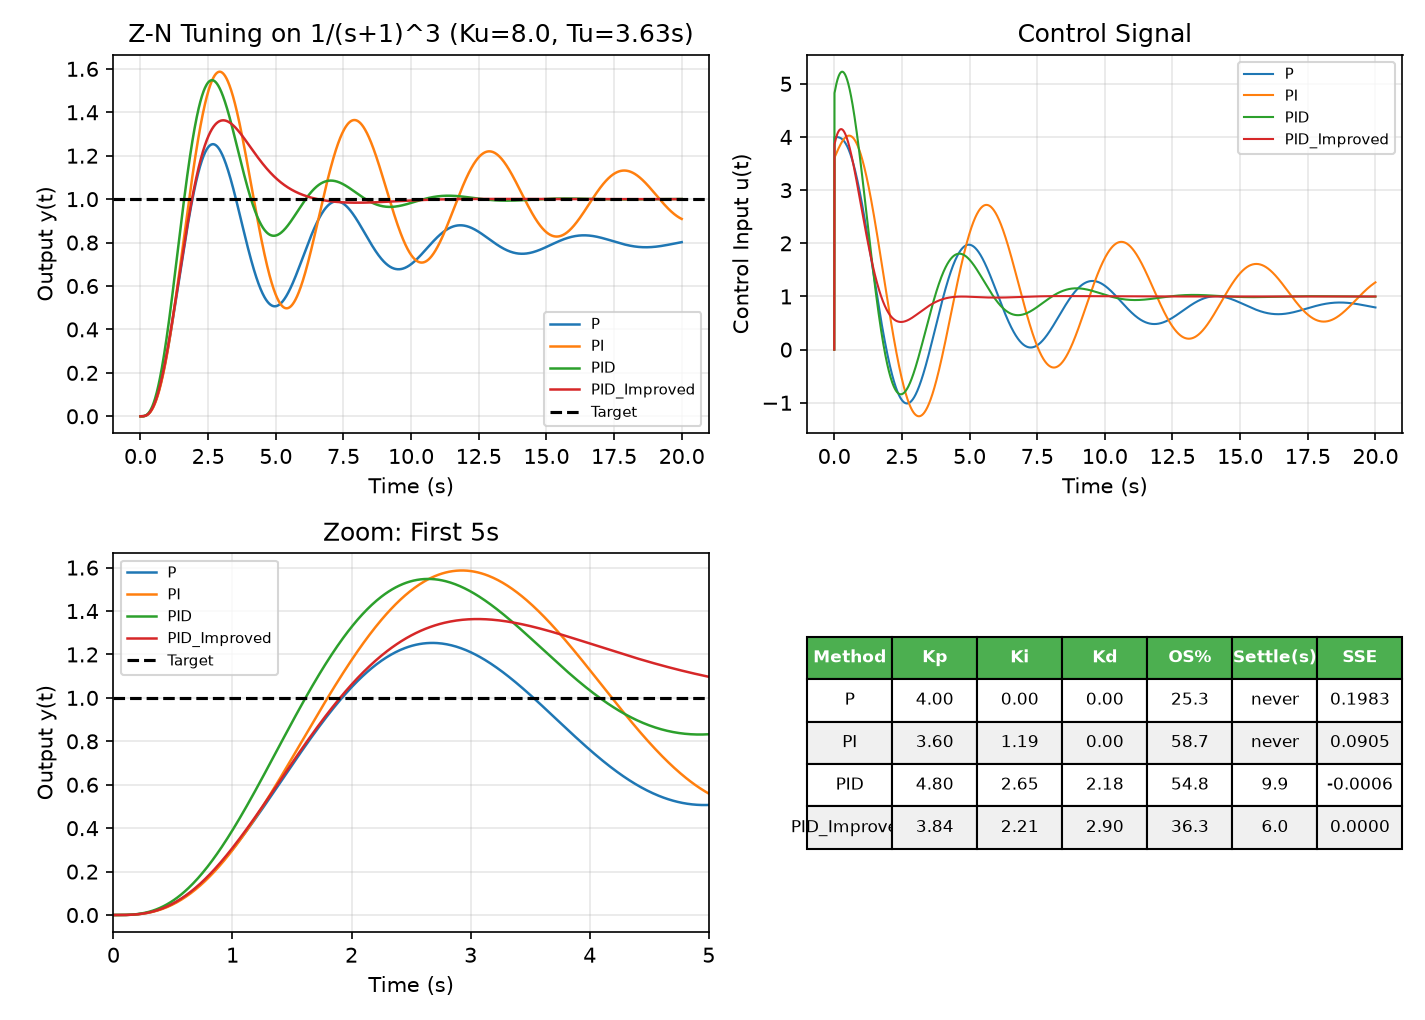
\includegraphics[width=0.78\linewidth]{../experiment_plots/exp5_zn_tuning.png}
		\caption{Step responses of $1/(s+1)^3$ using Ziegler--Nichols P, PI, PID, and the manually improved PID.}
		\label{fig:zn}
	\end{figure}
	
	\subsection{Manual tuning step by step}
	\begin{table}[h]
		\centering
		\small
		\begin{tabular}{@{}lllll@{}}
			\toprule
			Increase & Rise time & Overshoot & Settling time & Steady-state error \\
			\midrule
			$K_p$ & decreases & increases & small change & decreases (never zero alone) \\
			$K_i$ & decreases a little & increases & increases & removed \\
			$K_d$ & small change & decreases & decreases & no change \\
			\bottomrule
		\end{tabular}
		\caption{Independent effect of increasing each PID gain.}
	\end{table}
	
	Following the loop in Figure~\ref{fig:tuning}: (1) set $K_i=K_d=0$ and raise $K_p$ for a fast rise; (2) raise $K_d$ to damp overshoot (adding a low-pass filter if noisy); (3) raise $K_i$ slowly to eliminate steady-state error (enabling anti-windup if saturated); (4) iterate until specifications are met.
	
	\begin{figure}[h]
		\centering
		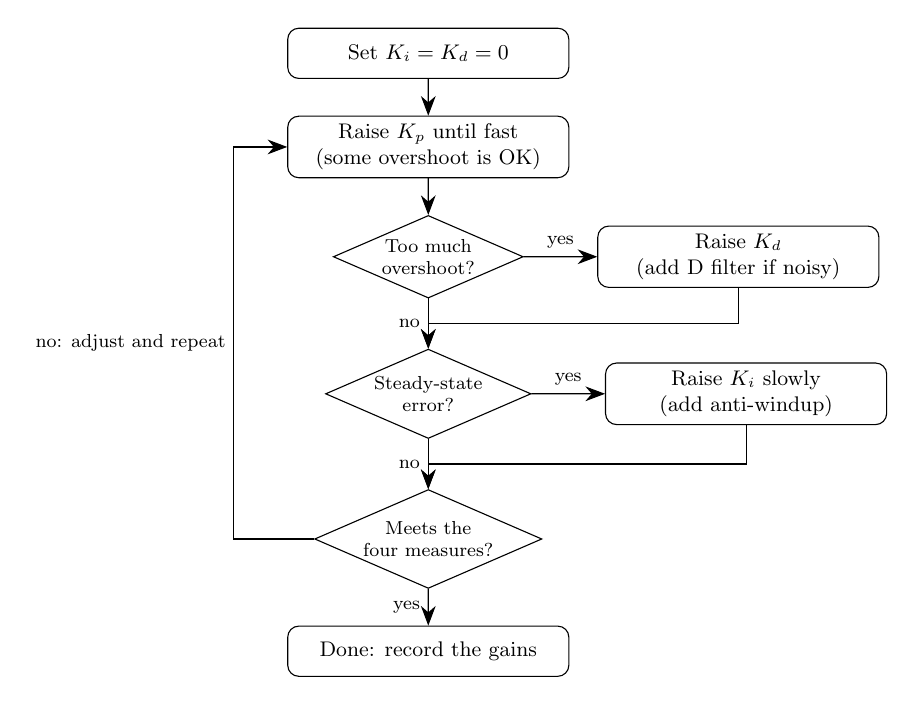
\begin{tikzpicture}[
			scale=0.85,
			transform shape,
			node distance=0.55cm,
			box/.style={draw, rectangle, rounded corners, align=center, minimum width=4.2cm, minimum height=0.75cm, font=\small},
			dec/.style={draw, diamond, aspect=2.3, align=center, inner sep=1pt, font=\footnotesize},
			>={Stealth[length=2.5mm]}
			]
			\node[box] (start) {Set $K_i = K_d = 0$};
			\node[box, below=of start] (kp) {Raise $K_p$ until fast\\(some overshoot is OK)};
			\node[dec, below=of kp] (os) {Too much\\overshoot?};
			\node[box, right=1.1cm of os] (kd) {Raise $K_d$\\(add D filter if noisy)};
			\node[dec, below=0.75cm of os] (sse) {Steady-state\\error?};
			\node[box, right=1.1cm of sse] (ki) {Raise $K_i$ slowly\\(add anti-windup)};
			\node[dec, below=0.75cm of sse] (ok) {Meets the\\four measures?};
			\node[box, below=0.55cm of ok] (done) {Done: record the gains};
			
			\draw[->] (start) -- (kp);
			\draw[->] (kp) -- (os);
			\draw[->] (os) -- node[above, font=\footnotesize] {yes} (kd);
			\draw[->] (os) -- node[left, font=\footnotesize] {no} (sse);
			\draw[->] (kd) |- ($(os.south)!0.5!(sse.north)$) -- (sse);
			\draw[->] (sse) -- node[above, font=\footnotesize] {yes} (ki);
			\draw[->] (sse) -- node[left, font=\footnotesize] {no} (ok);
			\draw[->] (ki) |- ($(sse.south)!0.5!(ok.north)$) -- (ok);
			\draw[->] (ok) -- node[left, font=\footnotesize] {yes} (done);
			\draw[->] (ok.west) -- ++(-1.2,0) |- node[pos=0.25, left, font=\footnotesize] {no: adjust and repeat} (kp.west);
		\end{tikzpicture}
		\caption{Step-by-step manual PID tuning workflow.}
		\label{fig:tuning}
	\end{figure}
	
	\subsection{Model-based tuning: grid search on the test system}
	Searching $K_p \in \{20,40,60,100,150,200\}$, $K_i \in \{50,100,150,200,300,400\}$, and $K_d \in \{0,2,5,10,15,20\}$ (216 combinations) with the 30\,N actuator clamp, anti-windup, and D-on-PV yields $K_p=100, K_i=400, K_d=5$ as the fastest valid controller ($M_p = 0.8\%$, $T_s = 0.62$\,s, down from $3.79$\,s with the un-tuned baseline).
	
	\subsection{Ziegler--Nichols on a second system}
	To tune without a plant model, we apply the Ziegler--Nichols (ZN) ultimate-sensitivity method to a third-order lag:
	\begin{equation}
		G(s) = \frac{1}{(s+1)^3}.
	\end{equation}
	With $K_i = K_d = 0$, raising $K_p$ produces sustained oscillations at the Routh--Hurwitz stability boundary $(s+1)^3 + K_p = 0 \implies 3 \cdot 3 = 1 + K_u$, giving:
	\begin{equation}
		K_u = 8.0, \qquad \omega_u = \sqrt{3}\ \text{rad/s}, \qquad T_u = \frac{2\pi}{\sqrt{3}} \approx 3.63\ \text{s}.
	\end{equation}
	
	\begin{table}[h]
		\centering
		\small
		\begin{tabular}{@{}lccc@{}}
			\toprule
			Controller & $K_p$ & $T_i$ & $T_d$ \\
			\midrule
			P   & $0.5\,K_u$  & ---       & --- \\
			PI  & $0.45\,K_u$ & $T_u/1.2$ & --- \\
			PID & $0.6\,K_u$  & $T_u/2$   & $T_u/8$ \\
			\bottomrule
		\end{tabular}
		\caption{Ziegler--Nichols tuning rules (where $K_i = K_p/T_i$ and $K_d = K_p\,T_d$).}
		\label{tab:zn_recipe}
	\end{table}
	
	Applying Table~\ref{tab:zn_recipe} yields aggressive responses with high overshoot (Table~\ref{tab:zn_results} and Figure~\ref{fig:zn}).
	
	Applying the standard ZN formulas ($P: 0.5K_u$; $PI: 0.45K_u, T_i=T_u/1.2$; $PID: 0.6K_u, T_i=T_u/2, T_d=T_u/8$) yields aggressive responses with high overshoot (Table~\ref{tab:zn_results} and Figure~\ref{fig:zn}). Following Section~8.1, lowering $K_p$ by $20\%$ ($0.48K_u = 3.84$), reducing $K_i$ ($1.0K_u/T_u = 2.21$), and raising $K_d$ ($0.1K_u T_u = 2.90$) cuts PID overshoot from $54.8\%$ down to $36.3\%$ while maintaining zero steady-state error.
	
	\begin{table}[h]
		\centering
		\small
		\begin{tabular}{@{}lrrrrrr@{}}
			\toprule
			Controller & $K_p$ & $K_i$ & $K_d$ & Rise time $T_r$ (s) & Overshoot $M_p$ (\%) & $e_{ss}$ (m) \\
			\midrule
			ZN P         & 4.00 & 0.00 & 0.00 & 1.14 & 25.3 & 0.1983 \\
			ZN PI        & 3.60 & 1.19 & 0.00 & 1.04 & 58.7 & 0.0905 \\
			ZN PID       & 4.80 & 2.65 & 2.18 & 0.93 & 54.8 & -0.0006 \\
			\midrule
			Improved PID & 3.84 & 2.21 & 2.90 & 1.12 & 36.3 & 0.0000 \\
			\bottomrule
		\end{tabular}
		\caption{Ziegler--Nichols gains and hand-improved PID performance on $G(s) = 1/(s+1)^3$.}
		\label{tab:zn_results}
	\end{table}
	

	
	\section{The Code}
	Below is the core Python implementation from \texttt{controllers.py}. Actuator saturation (\texttt{Clamp}) is handled inside the plant simulation loop rather than inside the PID function, ensuring clean separation between control logic and hardware physics:
	
	\begin{verbatim}
		def P(Kp, error):
				return Kp * error
		
		def D_filtered_pv(Kd, pv, previous_pv, dt, alpha, prev_filtered=0.0):
				derivative = (pv - previous_pv) / dt
				filtered_derivative = alpha * derivative + (1 - alpha) * prev_filtered
				return -Kd * filtered_derivative, filtered_derivative
		
		def I_anti_windup(Ki, error, dt, integral, min_val, max_val, u_raw):
				"""Integral term with conditional anti-windup."""
				# True Anti-Windup: Pause integration if saturated AND error is pushing further into saturation
				if (u_raw > max_val and error > 0) or (u_raw < min_val and error < 0):
						new_integral = integral
				else:
					new_integral = integral + error * dt
		
				i_term = Ki * new_integral
				return i_term, new_integral
		
		def PID_robust_all(Kp, Ki, Kd, error, pv, previous_pv, dt, integral,
		 min_val, max_val, alpha=0.1, prev_filtered=0.0):
				"""
				Fully robust PID = P + Anti-windup + D_filtered_pv
				"""
				p = P(Kp, error)
				d, new_filtered = D_filtered_pv(Kd, pv, previous_pv, dt, alpha, prev_filtered)
			
				i_term, new_integral = I_anti_windup(Ki, error, dt, integral, min_val, max_val, p + Ki * integral + d)
				u_requested = p + i_term + d
		
				return u_requested, new_integral, new_filtered
	\end{verbatim}
	
	Figure~\ref{fig:final} tests \texttt{PID\_robust\_all} against basic PID on the mass--spring--damper plant with all four real-world challenges active simultaneously ($\pm 30$\,N force limit, $\pm 1$\,mm sensor noise, a $1 \to 2$\,m target step at $t=5$\,s, and a slow $T_s=50$\,ms controller update). Note that at $2$\,m the spring requires $k r = 40$\,N, which exceeds the $30$\,N motor limit (capping steady-state position at $1.5$\,m, i.e., $e_{ss} = 0.50$\,m). While basic PID suffers violent saturation banging and derivative spikes at $t=5$\,s, Robust PID eliminates the derivative kick, prevents windup, and reduces control force chatter ($\text{std}$ drops from $5.34$\,N to $5.02$\,N).
	
	\begin{figure}[h]
		\centering
		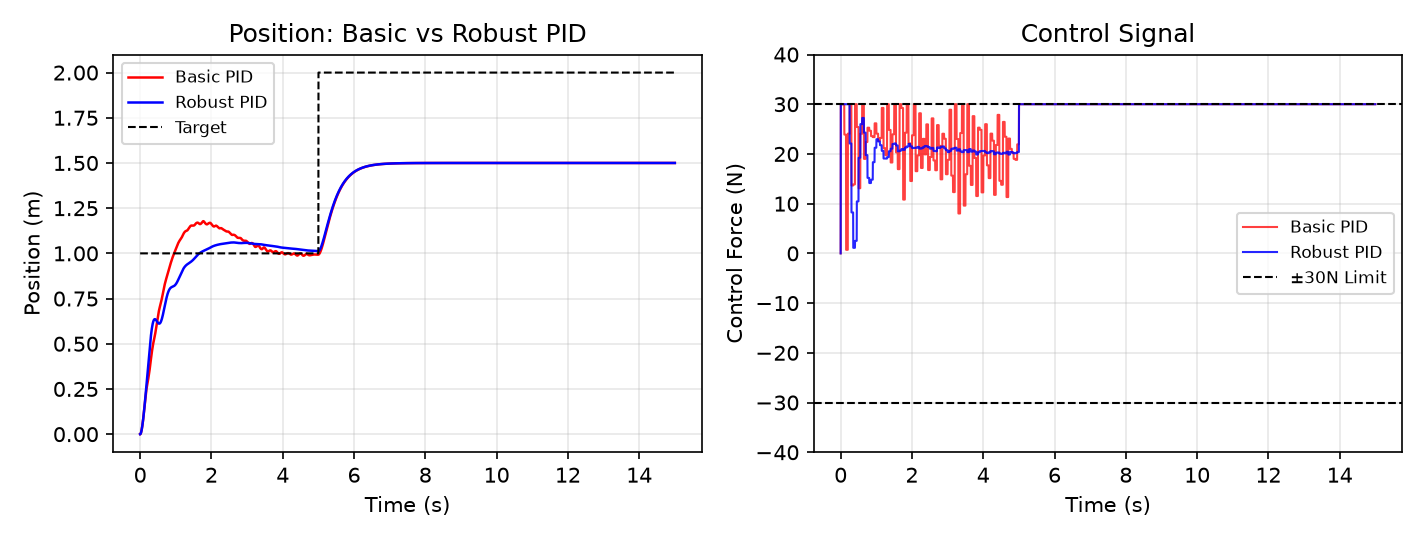
\includegraphics[width=0.82\linewidth]{../experiment_plots/exp6_final_comparison.png}
		\caption{Basic PID vs.\ Robust PID under simultaneous $\pm 30$\,N limit, $\pm 1$\,mm noise, $1 \to 2$\,m step at $t=5$\,s, and $T_s=50$\,ms update.}
		\label{fig:final}
	\end{figure}
	
	\section{Real Robots and Myths}
	PID loops appear wherever hardware must hold a setpoint against disturbances (Table~\ref{tab:examples}). Complex machines such as drones and robotic arms cascade multiple loops: an outer loop computes desired velocity or torque, and a faster inner loop regulates motor current or rotor speed.
	
	\begin{table}[h]
		\centering
		\small
		\begin{tabularx}{\textwidth}{llllX}
			\toprule
			Application & Setpoint / Sensor & Output & How PID helps \\
			\midrule
			DC motor speed & Target rpm / encoder & PWM voltage & P accelerates quickly; I eliminates steady speed droop under load. \\ \addlinespace
			Quadcopter drone & Roll, pitch, yaw / IMU & Rotor thrust & Separate attitude loops stabilize flight; D damps wind-gust wobble. \\ \addlinespace
			Robot arm joint & Joint angle / encoder & Motor torque & I holds constant torque to counteract gravity at any angle. \\ \addlinespace
			Line-following robot & Line center / IR array & Wheel speed diff & P steers onto the line; D prevents high-speed zig-zagging. \\ \addlinespace
			Car cruise control & Target speed / wheel sensor & Throttle & I maintains speed uphill where extra constant force is required. \\
			\bottomrule
		\end{tabularx}
		\caption{Real-world robotics and control applications of PID.}
		\label{tab:examples}
	\end{table}
	
	\subsection{Common myths about PID}
	\paragraph{Myth 1: ``Higher gains always give a better response.''}
	\emph{Reality:} Raising $K_p$ speeds up the initial response only up to a point; beyond it, overshoot and oscillation grow until the loop becomes unstable (as seen at $K_u = 8$ in Section~8.3).
	
	\paragraph{Myth 2: ``You always need all three terms.''}
	\emph{Reality:} Many industrial loops use PI only because D amplifies high-frequency sensor noise (Section~7.2), while simple systems with tolerable offset use P alone.
	
	\paragraph{Myth 3: ``The integral term fixes everything.''}
	\emph{Reality:} While I removes steady-state error, it adds phase lag and causes severe overshoot during actuator saturation unless anti-windup is implemented (Section~7.1).
	
	\paragraph{Myth 4: ``PID is the best controller for every problem.''}
	\emph{Reality:} PID excels on single-input, single-output systems, but multi-variable systems with strong coupling, strict state constraints, or long dead times benefit from LQR or Model Predictive Control (MPC).
	
	\paragraph{Myth 5: ``Once tuned, the gains are good forever.''}
	\emph{Reality:} Changes in payload mass, battery voltage, or mechanical wear shift plant dynamics, requiring periodic re-tuning or gain scheduling.
	
	\medskip
	\noindent\textit{Note on tools used:} Python (NumPy and Matplotlib) was used to simulate the differential equations and generate all figures. An AI assistant was used to help program the plotting code, refactor the codebase and format the LaTeX document.
	
\end{document}